\chapter{Ozadje in sorodna dela}

\section{Tehnologija LoRa}
LoRa je brezžična komunikacijska tehnologija, namenjena prenosu majhnih količin podatkov na velike razdalje ob zelo nizki porabi energije. Spada v razred tehnologij LPWAN (Low Power Wide Area Network), katerih glavni cilj je omogočiti povezljivost naprav interneta stvari v okoljih, kjer klasične brezžične tehnologije niso primerne zaradi dosega, porabe energije ali stroškov.

V primerjavi s tehnologijami, kot so Wi-Fi, Bluetooth ali mobilna omrežja, LoRa omogoča bistveno večji doseg ob večkrat nižji porabi energije, vendar na račun nizke hitrosti prenosa podatkov. Tipični scenariji uporabe vključujejo senzorje, merilne naprave in sledilnike, ki periodično pošiljajo majhne količine podatkov in morajo delovati več let brez menjave baterije.

\subsection{Tehnične značilnosti LoRa}

Na fizičnem sloju LoRa uporablja modulacijo razširjenega spektra s frekvenčnimi čirpi (angl. \emph{chirp spread spectrum}). Ta modulacija omogoča visoko občutljivost sprejemnika ter robustno komunikacijo tudi pri zelo nizkih razmerjih signal–šum (angl. \emph{signal-to-noise ratio}, SNR). Posledično lahko LoRa povezave dosegajo razdalje več kilometrov v urbanih okoljih in tudi več deset in sto kilometrov v ruralnih ali odprtih območjih. Pomembna lastnost tehnologije LoRa je visok radijski proračun (angl. \emph{link budget}), ki je posledica kombinacije nizkih frekvenc, nizkih oddajnih moči ter visoke občutljivosti sprejemnikov.~\cite{8474715}

\section{Orodja za načrtovanje brezžičnih omrežij}

Na področju načrtovanja brezžičnih omrežij obstaja več orodij, ki omogočajo simulacijo širjenja radijskega signala, oceno pokritosti ter analizo vidne linije. Večina obstoječih rešitev se osredotoča na posamezne vidike načrtovanja in ne ponuja celovitega pristopa, ki bi združeval vse ključne funkcionalnosti v eni aplikaciji. V nadaljevanju so predstavljena nekatera pomembnejša obstoječa orodja.

\subsection{Meshtastic Site Planner}
Meshtastic Site Planner~\cite{meshtasticSitePlanner} je odprtokodno orodje za modeliranje širjenja radijskega signala, ki temelji na uporabi programa SPLAT!~\cite{splatTool}. Orodje ponuja uporabniku prijazen spletni vmesnik ter osnovno vizualizacijo pokritosti na zemljevidu. Njegova glavna omejitev je pomanjkanje naprednejših funkcionalnosti, kot so analiza vidne linije ali optimizacija postavitev oddajnikov. Posledično je primeren predvsem za osnovno oceno pokritosti, ne pa za celovitejše načrtovanje omrežij. Poleg tega se rezultati simulacij v celoti prenašajo v brskalnik, kar lahko negativno vpliva na uporabniško izkušnjo pri zahtevnejših izračunih.

\begin{figure}[htb]
\centering
\includegraphics[width=1\textwidth]{fotografije/site-meshtastic-org-celni-sistem.png}
\caption{Posnetek zaslona čelnega sistema sorodnega dela site.meshtastic.org}
\label{fig:site-meshtastic-org}
\end{figure}

\subsection{Radio Mobile Online}
Radio Mobile Online~\cite{ve2dbeRFPathCalc} je spletno orodje, ki prav tako temelji na uporabi programa SPLAT!~\cite{splatTool} za izračun širjenja radijskega signala med oddajnikom in sprejemnikom. Omogoča simulacijo radijske pokritosti ob upoštevanju topografskih podatkov in osnovnih radijskih parametrov. Orodje odlikuje funkcionalnost, vendar ga omejujeta nekoliko zastarel uporabniški vmesnik ter omejene možnosti razširitve, saj ne omogoča enostavne integracije z drugimi sistemi ali dodajanja dodatnih analiznih funkcionalnosti.

\begin{figure}[htb]
\centering
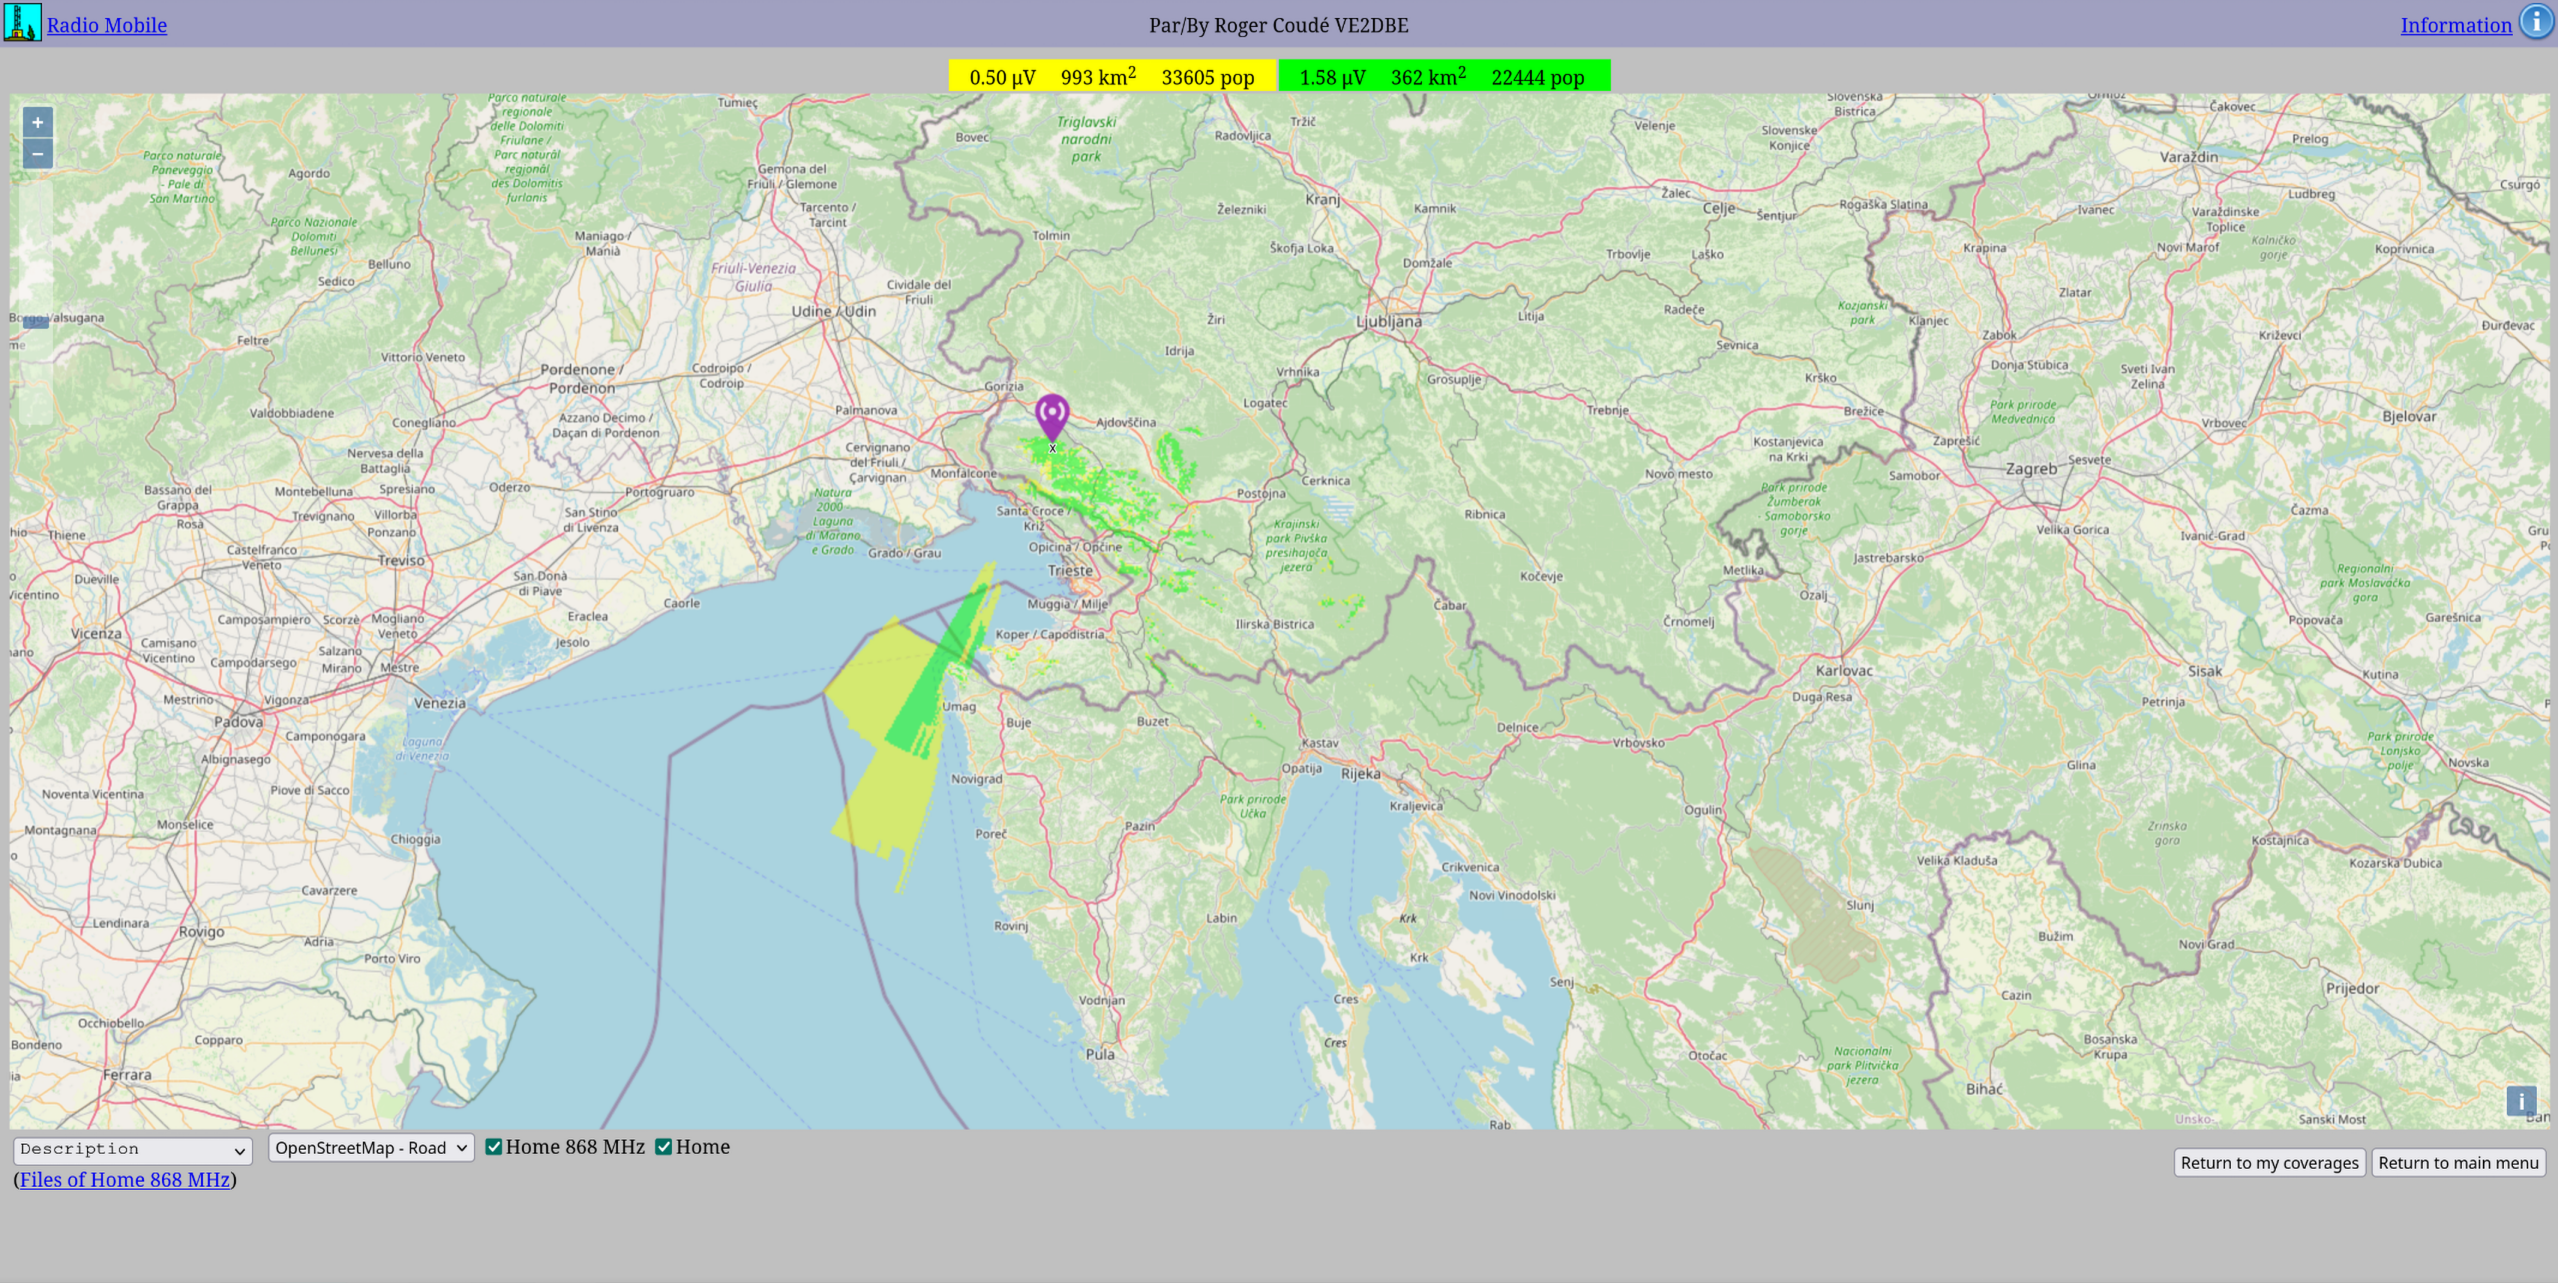
\includegraphics[width=1\textwidth]{fotografije/radio-mobile-online-celni-sistem.png}
\caption{Posnetek zaslona čelnega sistema sorodnega dela Radio Mobile Online}
\label{fig:radio-mobile-online}
\end{figure}

\subsection{SCADACore RF Line-of-Sight Calculator}
Orodje RF Line-of-Sight Calculator podjetja SCADACore~\cite{scadacoreRFLoS} je namenjeno preverjanju neposredne vidne linije med dvema točkama. Uporabniku omogoča hitro in enostavno oceno, ali med izbranima lokacijama obstaja neposredna vidna povezava. Kljub enostavni uporabi pa orodje ne podpira izračuna jakosti signala, analize Fresnelovih con ali vpliva frekvence, zato je uporabno predvsem kot informativno oziroma dopolnilno orodje.

\begin{figure}[htb]
\centering
\includegraphics[width=1\textwidth]{fotografije/scadacore-celni-sistem.png}
\caption{Posnetek zaslona čelnega sistema sorodnega dela SCADACore RF Line-of-Sight Calculator}
\label{fig:scadacore}
\end{figure}

\subsection{GRASS-RaPlaT}
RaPlaT (Radio Propagation and Terrain Analysis Tool)~\cite{raplatGrass,Ozimek2010GRASSRaPlaT} je odprtokodno orodje za modeliranje širjenja radijskega signala, ki temelji na geografskem informacijskem sistemu GRASS GIS. Omogoča uporabo različnih propagacijskih modelov nad prostorskimi podatki ter upošteva vpliv terena pri izračunu radijske pokritosti.

Glavna prednost orodja je njegova tesna integracija z GIS okoljem, ki omogoča natančno prostorsko analizo in uporabo različnih slojev geografskih podatkov. Njegova slabost pa je relativna zahtevnost uporabe, saj zahteva dobro poznavanje sistema GRASS GIS, dela z ukazno vrstico ter priprave prostorskih podatkov. Zaradi tega je RaPlaT primeren predvsem za raziskovalno in strokovno rabo, manj pa za hitro in intuitivno načrtovanje radijskih omrežij. Orodje prav tako ne ponuja neposredne analize vidne linije med poljubno izbranimi točkami.

\begin{figure}[htb]
\centering
\includegraphics[width=1\textwidth]{fotografije/ijs-raplat-celni-sistem.png}
\caption{Posnetek zaslona čelnega sistema sorodnega dela GRASS-RaPlaT}
\label{fig:raplat}
\end{figure}

Pregled sorodnih del pokaže, da obstoječa orodja praviloma ponujajo bodisi simulacijo pokritosti bodisi analizo vidne linije, redko pa oboje v integrirani in razširljivi obliki. Predstavljeno delo te omejitve naslavlja z združitvijo simulacij, vizualizacije in eksperimentalne evalvacije v enem odprtokodnem orodju.